% Standalone source of the figure fig:multipole of the continuum-limit paper: the Cartesian multipole
% hierarchy. Build: lualatex fig_multipole.tex (or pdflatex); the paper includes the PDF.
% Legible in grey scale: shading, line styles and markers only.
\documentclass[border=3pt]{standalone}
% Shared preamble of the continuum-limit paper's standalone figures.
\usepackage{amsmath,amssymb,bm}
\usepackage{tikz}
\usetikzlibrary{calc}
\newcommand{\bS}{\mathbf{S}}
\newcommand{\bG}{\mathbf{G}}
\newcommand{\bK}{\mathbf{K}}
\newcommand{\bP}{\mathbf{P}}
\newcommand{\sinc}{\operatorname{sinc}}

\usetikzlibrary{arrows.meta}
\begin{document}
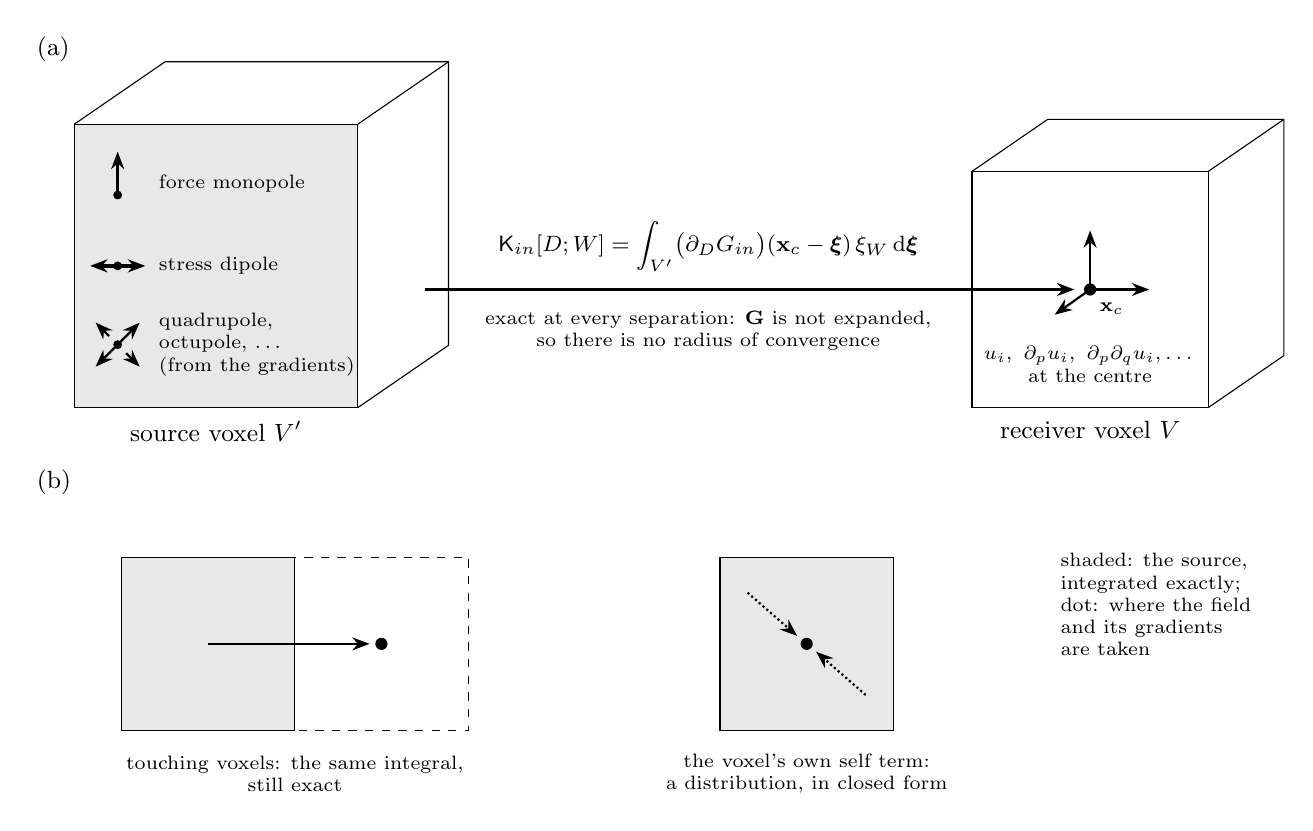
\begin{tikzpicture}[>={Stealth[length=2.2mm]}, font=\small]
  % a cube in oblique projection: front face at (#1,#2), side #3, front fill #4
  \newcommand{\cube}[4]{%
    \fill[#4] (#1,#2) rectangle ++(#3,#3);
    \draw (#1,#2) rectangle ++(#3,#3);
    \draw (#1,#2+#3) -- ++(0.32*#3,0.22*#3) -- ++(#3,0) -- ++(0,-#3) -- (#1+#3,#2);
    \draw (#1+#3,#2+#3) -- ++(0.32*#3,0.22*#3);
  }
  % ---------------------------------------------------------------- (a) two voxels apart
  \node[anchor=west] at (-0.6,4.55) {(a)};
  % source voxel
  \cube{0}{0}{3.6}{gray!18}
  \node[below] at (1.8,-0.05) {source voxel $V'$};
  % its multipole moments, drawn inside: monopole, stress dipole, quadrupole
  \fill (0.55,2.7) circle (1.6pt);
  \draw[->, very thick] (0.55,2.7) -- ++(0,0.55);
  \node[font=\scriptsize, anchor=west] at (0.95,2.85) {force monopole};
  \fill (0.55,1.8) circle (1.6pt);
  \draw[->, very thick] (0.55,1.8) -- ++(0.35,0);
  \draw[->, very thick] (0.55,1.8) -- ++(-0.35,0);
  \node[font=\scriptsize, anchor=west] at (0.95,1.8) {stress dipole};
  \fill (0.55,0.8) circle (1.6pt);
  \draw[->, thick] (0.55,0.8) -- ++(0.28,0.28);
  \draw[->, thick] (0.55,0.8) -- ++(-0.28,-0.28);
  \draw[<-, thick, dashed] (0.55,0.8) ++(0.28,-0.28) -- (0.55,0.8);
  \draw[<-, thick, dashed] (0.55,0.8) ++(-0.28,0.28) -- (0.55,0.8);
  \node[font=\scriptsize, anchor=west, align=left] at (0.95,0.8) {quadrupole,\\octupole, \dots\\(from the gradients)};
  % receiver voxel
  \cube{11.4}{0}{3}{white}
  \node[below] at (12.9,-0.05) {receiver voxel $V$};
  \fill (12.9,1.5) circle (2.2pt);
  \node[font=\scriptsize, below right] at (12.9,1.45) {$\mathbf x_c$};
  \draw[->, thick] (12.9,1.5) -- ++(0.75,0);
  \draw[->, thick] (12.9,1.5) -- ++(0,0.75);
  \draw[->, thick] (12.9,1.5) -- ++(-0.45,-0.32);
  \node[font=\scriptsize, align=center] at (12.9,0.55) {$u_i,\ \partial_pu_i,\ \partial_p\partial_qu_i,\dots$\\ at the centre};
  % the coupling
  \draw[->, line width=1.1pt] (4.45,1.5) -- (12.7,1.5);
  \node[above, align=center, font=\footnotesize] at (8.05,1.6)
    {$\mathsf K_{in}[D;W]=\displaystyle\int_{V'}\bigl(\partial_DG_{in}\bigr)(\mathbf x_c-\boldsymbol\xi)\,\xi_W\,\mathrm d\boldsymbol\xi$};
  \node[below, align=center, font=\scriptsize] at (8.05,1.35)
    {exact at every separation: $\mathbf G$ is not expanded,\\ so there is no radius of convergence};
  % ---------------------------------------------------------------- (b) where an expansion would fail
  \node[anchor=west] at (-0.6,-0.95) {(b)};
  % touching voxels
  \fill[gray!18] (0.6,-4.10) rectangle ++(2.2,2.2);
  \draw (0.6,-4.10) rectangle ++(2.2,2.2);
  \draw[dashed] (2.8,-4.10) rectangle ++(2.2,2.2);
  \fill (3.9,-3.00) circle (2.2pt);
  \draw[->, thick] (1.7,-3.00) -- (3.75,-3.00);
  \node[align=center, font=\scriptsize] at (2.8,-4.65) {touching voxels: the same integral,\\ still exact};
  % the self term
  \fill[gray!18] (8.2,-4.10) rectangle ++(2.2,2.2);
  \draw (8.2,-4.10) rectangle ++(2.2,2.2);
  \fill (9.3,-3.00) circle (2.2pt);
  \draw[->, thick, densely dotted] (8.55,-2.35) -- (9.18,-2.90);
  \draw[->, thick, densely dotted] (10.05,-3.65) -- (9.42,-3.10);
  \node[align=center, font=\scriptsize] at (9.3,-4.65) {the voxel's own self term:\\ a distribution, in closed form};
  % legend for the line styles
  \node[align=left, font=\scriptsize, anchor=west] at (12.4,-2.50)
    {shaded: the source,\\ integrated exactly;\\ dot: where the field\\ and its gradients\\ are taken};
\end{tikzpicture}
\end{document}
